% !TeX spellcheck = en_GB
% !TeX program = pdflatex
%
% LuxSleek-CV 1.1 LaTeX template
% Author: Andreï V. Kostyrka, University of Luxembourg
%
% 1.1: added tracking and letter-spacing for prettier lower caps, added `~` for language levels
% 1.0: initial release
%
% This template fills the gap in the available variety of templates
% by proposing something that is not a custom class, not using any
% hard-coded settings deeply hidden in style files, and provides
% a handful of custom command definitions that are as transparent as it gets.
% Developed at the University of Luxembourg.
%
% *NOTHING IS HARCODED, and never should be.*
%
% Target audience: applicants in the IT industry, or business in general
%
% The main strength of this template is, it explicitly showcases how
% to break the flow of text to achieve the most flexible right alignment
% of dates for multiple configurations.

\documentclass[11pt, a4paper]{article} 

\usepackage[T1]{fontenc}     % We are using pdfLaTeX,
\usepackage[utf8]{inputenc}  % hence this preparation
\usepackage[british]{babel}  
\usepackage[left = 0mm, right = 0mm, top = 0mm, bottom = 0mm]{geometry}
\usepackage[stretch = 25, shrink = 25, tracking=true, letterspace=30]{microtype}  
\usepackage{graphicx}        % To insert pictures
\usepackage{xcolor}          % To add colour to the document
\usepackage{marvosym}        % Provides icons for the contact details

\usepackage{enumitem}        % To redefine spacing in lists
\setlist{parsep = 0pt, topsep = 0pt, partopsep = 1pt, itemsep = 1pt, leftmargin = 6mm}

\usepackage{tgtermes}        % Change this to use any font, but keep it simple
\renewcommand{\familydefault}{\sfdefault}

\definecolor{cvblue}{HTML}{304263}

%%%%%%% USER COMMAND DEFINITIONS %%%%%%%%%%%%%%%%%%%%%%%%%%%
% These are the real workhorses of this template
\newcommand{\dates}[1]{\hfill\mbox{\textbf{#1}}} % Bold stuff that doesn’t got broken into lines
\newcommand{\is}{\par\vskip.5ex plus .4ex} % Item spacing
\newcommand{\smaller}[1]{{\small$\diamond$\ #1}}
\newcommand{\headleft}[1]{\vspace*{3ex}\textsc{\textbf{#1}}\par%
    \vspace*{-1.5ex}\hrulefill\par\vspace*{0.7ex}}
\newcommand{\headright}[1]{\vspace*{2.5ex}\textsc{\Large\color{cvblue}#1}\par%
     \vspace*{-2ex}{\color{cvblue}\hrulefill}\par}
%%%%%%%%%%%%%%%%%%%%%%%%%%%%%%%%%%%%%%%%%%%%%%%%%%%%%%%%%%%%

\usepackage[colorlinks = true, urlcolor = white, linkcolor = white]{hyperref}

\begin{document}

% Style definitions -- killing the unnecessary space and adding the skips explicitly
\setlength{\topskip}{0pt}
\setlength{\parindent}{0pt}
\setlength{\parskip}{0pt}
\setlength{\fboxsep}{0pt}
\pagestyle{empty}
\raggedbottom

\begin{minipage}[t]{0.33\textwidth} %% Left column -- outer definition
%  Left column -- top dark rectangle
\colorbox{cvblue}{\begin{minipage}[t][5mm][t]{\textwidth}\null\hfill\null\end{minipage}}

\vspace{-.2ex} % Eliminates the small gap
\colorbox{cvblue!90}{\color{white}  %% LEFT BOX
\kern0.09\textwidth\relax% Left margin provided explicitly
\begin{minipage}[t][293mm][t]{0.82\textwidth}
\raggedright
\vspace*{2.5ex}

\Large \textbf{\textsc{Tomás Borges}} \normalsize 

% Centering without extra vertical spacing
\null\hfill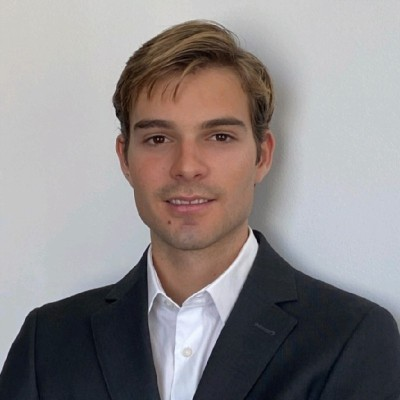
\includegraphics[width=0.65\textwidth]{pfp.jpeg}\hfill\null

\vspace*{0.5ex} % Extra space after the picture

\headleft{Profile}
Creative and goal-driven data analyst with 2+ years of experience in data science, specializing in data analysis, manipulation, modeling, and predictive analytics. Skilled in automating workflows, optimizing ETL processes, exploratory data analysis (EDA), and creating actionable insights through dynamic reports. Proficient in Python, SQL, and visualization tools like Power BI and Looker. Strong communicator with a proven ability to collaborate across teams and deliver data-driven solutions that support organizational goals.

\headleft{Contact details}
\small % To fit more content
\MVAt\ {\small tomasalmeidaborges@gmail.com} \\[0.4ex]
\Mobilefone\ +351\,964103096 \\[0.5ex]
\Mundus\ \href{https://github.com/TBorges99}{github.com/TBorges99} \\[0.1ex]
\Mundus\ \href{https://linkedin.com/in/taborges}{linkedin.com/in/taborges} \\[0.1ex]
\normalsize

\headleft{Fluent Languages}
%Year of birth: \textbf{1861} \\[0.5ex]
\textbf{Portuguese}~(native)
\textbf{English}~(fluent)

\headleft{Skills}
\begin{itemize}
\item Python (NumPy, Pandas, Scikit-learn, Matplotlib, Plotly, Seaborn, PMDArima, FastAPI, OpenAI API)
\item SQL
\item Looker (LookML)
\item Power BI (DAX)
\item F\#
\item Microsoft Excel Expert
\end{itemize} 

\end{minipage}%
\kern0.09\textwidth\relax%%Right margin provided explicitly to stretch the colourbox
}
\end{minipage}% Right column
\hskip2.5em% Left margin for the white area
\begin{minipage}[t]{0.56\textwidth}
\setlength{\parskip}{0.8ex}% Adds spaces between paragraphs; use \\ to add new lines without this space. Shrink this amount to fit more data vertically

\vspace{2ex}

\headright{Experience}

\textsc{Data Analyst} at \textit{Leadzai.}  \dates{Oct.2023--Present} \\
\smaller Led Business Intelligence (BI) initiatives by designing dynamic SQL reports, optimizing tables, and leveraging PDTs to transform raw PostgreSQL and BigQuery data into actionable insights. \\
\smaller Conducted Exploratory Data Analysis (EDAs) in Python to identify bottlenecks and optimize the AI-driven ad creation pipeline. \\
\smaller Developed robust LookML models and intuitive Looker dashboards, enabling teams to make confident, data-driven decisions in a fast-paced, constantly evolving startup environment. \\
\smaller Optimized ETL workflows, improving Data Warehouse efficiency and reducing costs.

\is % Item spacing -- defined in the preamble
\textsc{Data Science Trainee} at \textit{EDP Comercial.}  \dates{Nov.2022--Aug.2023} \\
\smaller Worked on diverse data science projects, including data analysis, modeling, predictive analytics, and data visualization. \\
\smaller Automated data collection procedures using Python, reducing operational time from 90 to 30 minutes, improving productivity and data reliability. \\
\smaller Built a Data Hub for energy market product prices, optimizing ETL processes and enabling BI dashboards. \\
\smaller Used web scraping techniques and API integrations to collect market, consumption, and production data. \\
\smaller Designed anomaly detection algorithms to improve data quality and enhance market price analysis.

\headright{Education}

\textsc{MSc in Finance.} (gpa: 17/20)   \textit{ Nova School of Business and Economics}. \dates{2020--2022} \\
\smaller{Thesis: \textit{Equity Research on Nvidia}} \\
\smaller{Specialization: \textit{Business and Data Analytics}}\\
\smaller{Relevant Courses: \textit{Machine Learning, Data Curation, Data
Visualisation, Data Analytics for Finance, Financial Econometrics, Risk Management.}}

\is
\textsc{BSc in Management.} \textit{ Nova School of Business and Economics}.  \dates{2017--2020} \\

\headright{Other Projects}
\smaller{Exploring FastAPI and OpenAI API: Recently developed an AI-driven application using FastAPI for backend development. The app's purpose is to assist with data cleaning and preprocessing (available on GitHub).} \\
\smaller{Built personal projects on regression, classification, and time-series forecasting (available on GitHub) such as building a model for forecasting electricity prices in Spain (achieving an RMSE of 2.47)} \\
\smaller{Participated in data science competitions (kaggle), focusing on data visualization and machine learning algorithms.} \\
\smaller{Managed a personal investment portfolio since 2020; active member of the Nova Social Investment Fund during MSc.}

\headright{Hobbies}

\smaller{\textit{Oil Painting \& Drawing:} I am an amateur artist who brings life to canvas and paper, having sold a few cherished works while honing my craft in drawing classes.}\\
\smaller{\textit{Hiking:} Avid hiker who enjoys adventures on the trails.}

\end{minipage}

\end{document}